\item \textbf{Energy and Power of a wave}
    \begin{center}
        \begin{tikzpicture}
            \tzfn"curve"{sin(deg(\x))}[0:pi]
            \tzfn[line width=0.5mm]{sin(deg(\x))}[0.2*pi:0.3*pi]
            \tzvXpointat*{curve}{pi*0.25}(A)
            \tzline+[->](A)(0, 0.5){$v_p$}[a]
            %\tzline+[->](A)(0, -0.5)
            \begin{scope}[xshift=6cm]
                \tzline+(0, 0)(2, 0){$\Delta x$}[mb]
                \tzline+(2, 0)(0, 0.5){$\Delta y$}[mr]
                \tzline(0, 0)(2, 0.5){$\Delta l$}[ma]
            \end{scope}
        \end{tikzpicture}
    \end{center}
    \begin{center}
        \begin{quote}
            \textit{In the context of a string wave, consider the movement of a segment of the string. As this segment oscillates, it possesses kinetic energy, quantifiable by the formula $\dfrac{1}{2}mv^2$. However, there is an additional phenomenon at play: the string segment also undergoes slight elongation, resulting in potential energy. Each element behaves as a temporary spring, and the potential energy can be calculated using $\int\vec{F}\cdot\d{\vec{s}}$. The total energy of the segment is the sum of the kinetic and potential energies.}
        \end{quote}
        \[ y(x, t) = A\sin\left(kx-\omega t\right) \]
    \end{center}
    \begin{align*}
        \intertext{Kinetic energy of the segment,}
        K.E. &= \dfrac{1}{2}m v_p^2 \\
            &= \int \dfrac{1}{2}\d{m}\left(\dfrac{\partial y}{\partial t}\right)^2\\
            &= \dfrac{1}{2}\left(\upmu\d{x} \right)\left(\dfrac{\partial y}{\partial t}\right)^2\\
            &= \int \dfrac{1}{2} \upmu A^2\omega^2 \cos^2\left(kx-\omega t\right) \d{x}\\
        \intertext{We can calculate average kinetic energy over one complete oscillation,}
        <K.E.> &= \dfrac{1}{2} \upmu A^2\omega^2\int_0^\lambda \cos^2\left(kx-\omega t\right) \d{x}\\ 
                &=\dfrac{1}{2} \upmu A^2\omega^2\int_0^\lambda \dfrac{\left(1 + \cos\left(2\left(kx-\omega t\right)\right)\right)}{2} \d{x}\\  
                &= \dfrac{1}{4} \upmu A^2\omega^2 \left[x + \dfrac{\sin\left(2kx-2\omega t\right)}{2k}\right]_0^\lambda\\
                &= \dfrac{1}{4} \upmu A^2\omega^2 \left[\lambda + \dfrac{\sin\left(2k\lambda-2\omega t\right)-\sin\left(-2\omega t\right)}{2k}\right]\\
                &= \dfrac{1}{4} \upmu A^2\omega^2 \left[\lambda + \dfrac{\sin\left(4\pi-2\omega t\right)+\sin\left(2\omega t\right)}{2k}\right]\\  
                &= \dfrac{1}{4} \upmu A^2\omega^2 \left[\lambda + \dfrac{2*\sin\left(2\pi\right)*\cos\left(4\pi-4\omega t\right)}{2k}\right]\\ 
                &= \dfrac{1}{4} \upmu A^2\omega^2 \lambda
    \end{align*}
    \pagebreak
    \begin{align*}
        \intertext{Potential energy of the segment,}\\
        \intertext{Firstly, we have to calculate the elongation in the segment using above right diagram}
        \Delta l &= \sqrt{\Delta x^2 + \Delta y^2} - \Delta x\\
            &= \Delta x\sqrt{1 + \left(\dfrac{\Delta y}{\Delta x}\right)^2} - \Delta x
            \intertext{As string will perform small oscillations $\dfrac{\Delta y}{\Delta x}$ will be small}
            &= \Delta x \left(1+\dfrac{1}{2} \left(\dfrac{\Delta y}{\Delta x}\right)^2\right) - \Delta x\\
        \Delta l &\approx \dfrac{1}{2}\left(\dfrac{\Delta y}{\Delta x}\right)^2 \Delta x
    \end{align*}
    \begin{align*}
        \intertext{As $\dfrac{\Delta y}{\Delta x}$ is slope hence, $\dfrac{\partial y}{\partial x}$,}
        U &= \int T \cdot \dfrac{1}{2} \left(\dfrac{\partial y}{\partial x}\right)^2 \d{x}\\
        &= \int \dfrac{1}{2} T A^2k^2 \cos^2\left(kx-\omega t\right) \d{x}\\
        \intertext{Again, we can calculate average potential energy over one complete oscillation,}
        <U> &= \dfrac{1}{2}TA^2k^2\int_0^\lambda  \cos^2\left(kx-\omega t\right) \d{x}
        \intertext{From above integration we got $\lambda/2$ and $\omega = \sqrt{\dfrac{T}{\upmu}}k$}
        <U> &= \dfrac{1}{4}\upmu A^2\omega^2\lambda
        \intertext{So, total energy in one complete oscillation will be,}
        \textit{Total Energy} &= K.E. + U\\
        \Aboxed{E &= \dfrac{1}{2}\upmu A^2\omega^2 \lambda}
        \intertext{Total energy per unit length will be like,}
        \dfrac{E}{\lambda} &= \dfrac{1}{2}\upmu A^2\omega^2\\
        \Aboxed{u &= \dfrac{1}{2}\upmu A^2\omega^2}
    \end{align*}
